\documentclass[12pt,fleqn]{article}\usepackage{../../common}
\begin{document}
Kalman Filtreleri

Diyelim ki bir video kameradan gelen imajları kullanarak obje takip eden bir
yazılım istiyoruz. Matematiksel olarak obje nedir? İmajı nedir? obje kendi
dünyasında bir süreci takip etmektedir, 3 boyutlu uzayda bir yer kaplamaktadır
ve orada hareket etmektedir. Biz bu hareketi belli bir güven aralığı / hata payı
üzerinden biliyor olabiliriz. Diğer yandan objenin kameraya yansıttığı imaj
vardır, bu imaj 2 boyutlu ve kameranın özellikleriyle alakalı parametreler
sebebiyle belli bir şekilde ``yansıtılmış (project)'' olacaktır. Biz bu yansıtma
formülünü de, belli bir hata payı üzerinden, biliyor olabiliriz.

Bu durumu şöyle modelleyebiliriz,

$$ x_k = \Phi_{k-1}x_{k-1} + w_{k-1} $$

$$ z_k = H_k x_k + v_k $$

$x_k = (n \times 1)$ vektörü, $k$ anındaki sürecin durumu (state)

$\Phi_k = (n \times n)$ matrisi, $x_{k-1}$ durumundan $x_{k}$ durumuna
geçişi tarif eden formül.

$w_k = (n \times 1)$ vektörü, sıfır ortalamalı, kovaryansı $Q_k$ olan beyaz
gürültü.

$z_k = (n \times 1)$ vektörü, dışarıdan alınan ölçüm.

$H_k = (m \times n)$ matrisi, gizli konum bilgisinin dışarıya nasıl ölçüm olarak
yansıdığının formülü. Bu dönüşüm ideal, yani gürültüsüz durumu tarif eder.

$v_k = (m \times 1)$ vektörü, ölçüm hatası.

Yani formüllerin söylediği şudur: ilk formül bize izlenen her ne ise onun
hareketini tarif ediyor, $k-1$ anından $k$ anına geçişini tarif ediyor. $z_k$
ise bu $x_k$'nin dışarıdan alınan ölçümü. Bizim yapmak istediğimiz $z_k$'leri
kullanarak $x_k$'nin nerede olduğunu kestirebilmek.

Sıfır merkezli gürültü şu demektir,

$$ E[v_k] = E[w_k] = 0 $$

Ayrıca,

$$ E[v_kv_k^T] = R_k $$

$$ E[w_kw_k^T] = Q_k $$

Kalman filtreleri (KF) ile yapmak istediğimizin dışarıdan görünen $z_k$'yi
kullanarak gizli $x_k$'yi kestirmek olduğunu söylemiştik. Ayrıca bu tahminleri
her gelen veri noktasına göre sürekli güncelliyor olacağız, yani 100 tane veri
noktasını almak için bekleyip sonra toptan bir analiz yapmaya gerek yok
(istenirse yöntem toptan işleyecek şekilde de kullanılabilir tabii). Tahmin
edilebileceği üzere bu tür bir gerçek zamanlı kabiliyetin pek çok mühendislik
uygulaması olabilir; hakikaten de mesella aya ilk insanlı ınışı yapan Apollo
modülü bir Kalman filtresi kullanıyordu.

KF'i türetmek için önce bir lineer tahmin edici (estimator) tanımlamak gerekir,
ve sonra bu tahmin ediciyi optimize eden şartların ne olduğu incelenir. Şu
notasyonu kullanalım: Tilde yani $\tilde{x}$ üzerindeki işaret, o değişkenin
tahmin ile gerçeği arasındaki hatayı temsil etmesi içindir, $\hat{x}$ üzerindeki
şapka ise istatistik dersinden hatırlayacağımız üzere tahmin edici
(estimator). Ayrıca bir değişkenin üzerindeki $^-$ ve $^+$ işaretlerini bu
değişkenin ölçüm dikkate alındıktan önceki ve sonraki (o sırayla) hali olarak
tanımlayalım.

Konum bilgisi ve hata arasındaki ilişkiyi şu şekilde belirtelim,

$$ \hat{x}_k^+ = x_k + \tilde{x_k}^+ $$

$$ \hat{x}_k^- = x_k + \tilde{x_k}^- $$

Elimizdeki en iyi tahmin $\hat{x}_k^-$'i yeni veri / ölçüm elde ettikten sonra
güncellemek istiyoruz. Bunu yaparken gürültülü ölçümle eldeki en son tahmini
lineer bir şekilde birleştirmek istiyoruz. Bu birleştirmeyi,

$$ \hat{x}_k^+ = \hat{x}_k^- + K_k (z_k - H_k \hat{x}_k^-)   $$

olarak temsil edebiliriz, $\hat{x}_k^+$ güncellenmiş tahmindir, $K_k$ ise
birleştirme faktörüdür (blending factor), ki bu değerin ne olduğunu şu anda
bilmiyoruz.

Tekrar düzenlersek, 

$$= \hat{x}_k^- - K_kH_k\hat{x}_k^- + K_kz_k    $$

$$ \hat{x}_k^+ = \hat{x}_k^- (I - K_kH_k) + K_kz_k $$

Daha temiz olması için $K_k' = I - K_kH_k$ diyelim, ve en baştaki
formülleri bir daha alta alta yazalım,

$$ 
\hat{x}_k^+  = K_k' \hat{x}_k^- + K_kz_k  
\mlabel{1}  
$$

$$ 
z_k = H_k x_k + v_k 
\mlabel{2} 
$$

$$ 
\hat{x}_k^+ = x_k + \tilde{x_k}^+ 
\mlabel{3} 
$$

$$ 
\hat{x}_k^- = x_k + \tilde{x_k}^- 
\mlabel{4}
$$

(1) içine (2)

$$ \hat{x}_k^+ = K_k' \hat{x}_k^- + K_k(H_k x_k + v_k)   $$

Eşitliğin solunu (3) ile açalım,

$$ x_k + \tilde{x_k}^+ = K_k' \hat{x}_k^- + K_k(H_k x_k + v_k)   $$

ve $x_k$'yi sağa geçirelim,

$$ \tilde{x_k}^+ = K_k' \hat{x}_k^- + K_k(H_k x_k + v_k) - x_k   $$

$\hat{x}_k^-$ yerine (4)

$$  = K_k' (x_k + \tilde{x_k}^-) + K_k(H_k x_k + v_k) - x_k   $$

$x_k$'leri yanyana getirip gruplayalım,

$$  = K_k' x_k + K_kH_k x_k  - x_k + K_k'\tilde{x_k}^- + K_kv_k   $$

$$ \tilde{x_k}^+ = x_k (K_k' + K_kH_k - I) + K_k'\tilde{x_k}^- + K_kv_k   $$

Üstteki tüm ifadenin beklentisini aldığımız zaman,

$$ E[\tilde{x_k}^+] = E[x_k (K_k' + K_kH_k - I)] + E[K_k'\tilde{x_k}^-] + E[K_kv_k]  $$

olacak değil mi? Burada biraz duralım, ve yansızlık kavramını düşünelim. Eğer
tahmin edici $\hat{x}^+$ yansız (unbiased) olsun istiyorsak, bu şu anlama gelir,

$$ E[\hat{x_k}^+] = E[x_k] $$

Düzenleyelim,

$$ E[\hat{x_k}^+] - E[x_k] = 0$$

$$ E[\hat{x_k}^+ - x_k] = 0$$

$$ E[ \tilde{x_k}^+] = 0$$

Şimdi, formülü son bıraktığımız yere dönelim, orada eğer $E[\tilde{x_k}^+]=0$
olsun istiyorsak ve $E[\tilde{x_k}^-] = 0$'in da doğru olduğu durumda geriye tek
kalan $K_k' + K_kH_k - I$ ifadesinin sıfır olmasıdır (çünkü $E[v_k]=0$ olacak
zaten), bu durumda herhangi bir $x_k$ için beklentinin sıfır gelmesi

$$ K_k' + K_kH_k - I = 0 $$

olmasına bağlıdır. Tabii o doğru ise,

$$ K_k' = I - K_kH_k  $$

Bu ifadeyi geriye, (1)'deki tahmin edicinin içine koyarsak

$$ \hat{x}_k^+  = (I - K_kH_k ) \hat{x}_k^- + K_kz_k  $$

Ya da 

$$ \hat{x}_k^+  = \hat{x}_k^- + K_k(z_k - H_k\hat{x}_k^- )  $$

Eğer $\hat{x}_k^-$ için (4) kullanırsak,

$$ \hat{x}_k^+  =  (x_k + \tilde{x_k}^-) + K_k(z_k - H_k( x_k + \tilde{x_k}^-) )  $$

Tekrar gruplama, 

$$ \hat{x}_k^+  =  \tilde{x_k}^- (I - K_kH_k) + x_k + K_k(z_k - H_kx_k)   $$

Ve (2)'yi $z_k - H_kx_k$ için kullanalım,

$$ \hat{x}_k^+ - x_k =  (I - K_kH_k)\tilde{x_k}^- + K_kv_k   $$

$$ \tilde{x}_k^+ = (I - K_kH_k)\tilde{x_k}^- + K_kv_k   $$

Böylece tekabül eden tahmin hatasını hesaplamış olduk. 

Tanım

$$ P_k^+ = E[ \tilde{x_k}^+\tilde{x_k}^{+T} ]$$

$$ P_k^- = E[ \tilde{x_k}^- \tilde{x_k}^{-T} ]$$

Bu kovaryans hesabının uygulanmasından ibaret aslında. Şimdi üç üstteki formülü
üstten ikincisine sokarsak,

$$ =  E \big[ (I - K_kH_k)\tilde{x_k}^- + K_kv_k \big] \big[\tilde{x_k}^{-T}(I - H_k^TK_k^T) + v_k^TK_k^T \big] $$

Yani

$$ 
= E \bigg[ (I - K_kH_k)\tilde{x_k}^- \big( \tilde{x_k}^{-T}(I - H_k^TK_k^T)
+ v_k^TK_k^T \big) + 
\mlabel{5}
$$

$$ K_kv_k \big( \tilde{x_k}^{-T}(I - H_k^TK_k^T) + v_k^TK_k^T  \big) \bigg] $$

Önceden tanımlamıştık,

$$ P_k^- = E[ \tilde{x_k}^- \tilde{x_k}^{-T} ]$$

$$ E[v_kv_k^T] = R_k $$

Ayrıca ölçüm hataları ve gürültü arasında korelasyon olmadığını farz ettiğimiz
için,

$$ E[\tilde{x_k}^-v_k^T] = E[v_k\tilde{x_k}^{-T}] = 0 $$

Tüm bunları (5)'i basitleştirmek için kullanırsak,

$$ 
P_k^{+} =  (I - K_kH_k)P_k^-(I - H_k^TK_k^T) + K_kR_kK_k^T 
\mlabel{6}
$$

En optimal $K_k$'yi nasıl buluruz? Amaç $P_k^+$ matrisinin çaprazındaki
değerleri minimize etmektir, bu durumda optimize etmek istediğimiz bedel (cost)
fonksiyonu

$$ J_k = E[ \tilde{x_k}^{+T}\tilde{x_k} ] $$

olsun, ki bu tek bir sayısal değer verir. Bu aslında 

$$ J_k = Tr(P_k^+) $$

değerinin optimize edilmesi ile aynı şeydir. Değil mi? Ya iki üstteki gibi
vektör uzunluğunu minimize ediyoruz, ya da kovaryansın çaprazının izini (trace)
minimize ediyoruz, çünkü her ikisinde de aynı değerler var. İz operatörü
hatırlayacağımız üzere bir matrisin çaprazındaki değerleri toplar. İz
kullanmamızın sebebi bize bazı türevsel numaralar sağlaması,

Biliyoruz ki, eger $B$ simetrik ise,

$$ \frac{\partial }{\partial A} Tr(ABA^T) = 2AB $$

$$ Tr(P_k^{+}) =  Tr((I - K_kH_k)P_k^-(I - H_k^TK_k^T)) + Tr(K_kR_kK_k^T) $$

İki tane iz var, bu izler içinde bir $ABA^T$ formu görebiliyoruz herhalde,
onların $K_k$'ye göre türevini alıyoruz,

$$ 
\frac{\partial Tr(P_k^{+})}{\partial K_k}  =
-2(I - K_kH_k)P_k^- H_k^T + 2K_kR_k
$$

Şimdi sıfıra eşitleyip $K_k$ için çözelim,

$$ 0 = -2(I - K_kH_k)P_k^- H_k^T + 2K_kR_k $$

$$  2P_k^- H_k^T = 2K_kH_kP_k^- H_k^T + 2K_kR_k $$

$$  P_k^- H_k^T = K_kH_kP_k^- H_k^T + K_kR_k  $$

$$  P_k^- H_k^T = K_k(H_kP_k^- H_k^T + R_k)  $$

$$  K_k = P_k^- H_k^T(H_kP_k^- H_k^T + R_k)^{-1} $$

$K_k$ matrisine Kalman kazanç matrisi (Kalman gain matrix) ismi de verilir. Ve
en son olarak bu sonucu (6) içine koyarsak, ve biraz manipülasyon ardından,

$$ P_k^+ = P_k^- -P_k^- H_k^T (H_kP_k^- H_k^T + R_k)^{-1}H_kP_k^-  $$

$$ = [I - K_kH_k]P_k^-  $$

sonucunu elde ederiz. 

Bu hesaplar ölçüm aldıktan {\em sonra} tahmini güncellemek içindi. Peki ölçüm
almadan önceki tahmini nasıl yaparız? Bunu yapmamız gerekir çünkü ölçüm gelmeden
önce yeni bir tahmin yapılmalı ki o tahmini, onun hatasını bir sonraki ölçüm ile
düzeltilebilelim. Bu geçişin nasıl olacağını en başta belirttiğimiz KF modeli
gösteriyor zaten, konum geçişi / adımı ona göre atıp, sonucun beklentisini ve
kovaryansını hesaplıyoruz,

$$ \hat{x}_k^- = E[\Phi_{k-1}x_{k-1}^+ + w] = \Phi_{k-1}x_{k-1}^+ $$

$$ P_k^- = Cov(\Phi_{k-1}x_{k-1}^+) = E[(\Phi_{k-1}x_{k-1}^+ + w)(\Phi_{k-1}x_{k-1}^+ + w)^T) $$

$$ =  \Phi_{k-1}P_{k-1}^+\Phi_{k-1}^T + Q_{k-1}  $$

$P_k^-$ hesabında ne olduğuna dikkat, bir sonraki ölçüm olmadan sadece geçiş
  formülü üzerinde tahmin etmeye uğraştık, ve bu tabii ki bilinmezliği arttırdı
  ($Q$ toplanıyor).

En son adım bu; $\hat{x}_k^-,P_k^-$ artık bir sonraki güncelleme için
kullanılacak değerlerdir. Bu noktada başa dönüyoruz, ve aynı işlemleri
tekrarlıyoruz. Eğer verinin alımı, model güncellemesi, ileri tahmin adımında
olanları bir figürle göstermek gerekirse (indisler resimde bir ileri alınmış,
bunu aklımızda düzelterek bakalım),

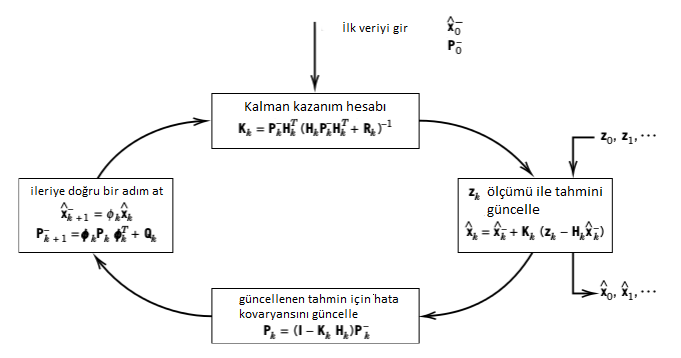
\includegraphics[height=8cm]{tser_kf_01.png}

Aslında tüm bu süreci bir sözde kod (pseudocode) parçası ile göstermeyi
düşünmüştük, ki ölçüm verisi bir \verb!for! döngüsü ile listeden alınarak teker
teker işlenecekti, fakat bu üstteki tarifi tam anlatamayacaktı, çünkü KF için
illa elde belli sayıda ``işlenip bitirilen'' ölçüm olması gerekmez. Güncelleme
her yeni ölçüm için, o tek ölçüm bazında yapılabildiği için şimdi 1 tane, sonra
10 tane, sonra bekleyip 2 tane daha, vs. şeklinde veri işlenmesi gayet
mümkündür. Bu işlem gerçek zamanlı olabilir, ya da bir listeyi gezerek anlık
olmayan bir şekilde olabilir.  Bu yüzden üstteki döngü resmini tercih ettik.

Not: Bazı kaynaklarda Kalman Filtrelerinin uygun bir model üzerinden en az
kareler (least square) ile yani çizgi / düzlem uydurması ile aynı sonuca
varabileceği söylenir, bu tam doğru degil, KF üstel ağırlıklı
(exponentially weighted) en az kareler ile aynıdır, yani en son veri
noktalarının daha öncekilere göre daha çok ağırlığı vardır. KF ile
regresyon örneği için bkz [5] yazısı.

Bir not daha: $x_k = \Phi_{k-1}x_{k-1} + w_{k-1}$ geçişinde $\Phi_{k-1}$
ile çarpım bir lineer konum değişimini modeller, o zaman lineer olmayan
geçişlerin KF modellenmesi mümkün değildir. Mesela bir topun ileri, havaya
doğru atıldığı bir örneği düşünelim, ölçümlerde Gaussian gürültü
olsun. Topun gidişi bir parabolu takip edecektir, oldukca basit bir
gidiştir, fakat KF'in bu gidişi takip etmesi mümkün değildir. Parçacık
filtreleri, genişletilmiş KF (EKF), UKF gibi yaklaşımlar bu sebeple
alternatif haline gelmişlerdir.

Bir KF kodlaması alttadır. 

\inputminted[fontsize=\footnotesize]{python}{kalman_3d.py}

Örnek

Diyelim ki tek boyutta bir köpeğin gidişini modellemek istiyoruz [4,
pg. 191]. Köpek sabit bir hızda ilerliyor olsun (bu geçiş modeli), ve biz
onu sadece havlamaların nereden geldiği ile bulmaya uğraşacağız (bu da
gürültülü ölçüm). Geçiş

$$ x = v \Delta t + x_0$$

Hız $v$ yerine $\dot{x}$ kullanalım, o zaman 

$$\bar x = x + \dot x \Delta t$$

Hız sabit olacağı için onun geçişi şöyle,

$$\bar{\dot x} = \dot x$$

Alt alta yazalım,

$$\begin{cases}
\begin{aligned}
\bar x &= x + \dot x \Delta t \\
\bar{\dot x} &= \dot x
\end{aligned}
\end{cases}$$

Düzenlersek,

$$\begin{cases}
\begin{aligned}
\bar x &= 1x + &\Delta t\, \dot x \\
\bar{\dot x} &=0x + &1\, \dot x
\end{aligned}
\end{cases}$$

Matris formunda

$$\begin{aligned}
\begin{bmatrix}\bar x \\ \bar{\dot x}\end{bmatrix} &= \begin{bmatrix}1&\Delta t  \\ 0&1\end{bmatrix}  \begin{bmatrix}x \\ \dot x\end{bmatrix}\\
\end{aligned}$$

$$ \mathbf{\bar x} = \mathbf{Fx} $$

Yani konumu iki boyutlu olarak modellemiş olduk.

$$\mathbf x =\begin{bmatrix}x \\ \dot x\end{bmatrix}$$

Peki ölçüm tahminlerini üretecek $H$ nasıl olmalı? 

$$\mathbf H=\begin{bmatrix}1&0\end{bmatrix}$$

Bunu yaptık çünkü $Hx$ çarpımı yapılınca sadece $x$ çarpıma girecek, hız
sıfırlanacak, yani ölçümde kullanılmayacak. Bu tam istediğimiz şey
zaten. Ne kadar ilginç değil mi? Hız konumda yer alan bir şey, tahmin /
ölçüm / düzeltme döngüsü sırasında KF onu da değiştirecek, düzeltecek,
ölçümde kullanılmıyor olsa bile! 

Ölçümdeki belirsizliğe 10 metre diyelim, 

$R = \begin{bmatrix}10\end{bmatrix}$

Altta alternatif bir KF kodu ve örneğin kodlamasını görüyoruz,

\inputminted[fontsize=\footnotesize]{python}{kalman.py}

\begin{minted}[fontsize=\footnotesize]{python}
from scipy.stats import norm, multivariate_normal
import pandas as pd, math
import numpy as np, numpy.linalg as linalg
import matplotlib.pyplot as plt
import kalman

def pos_vel_filter(x, P, R, Q=0., dt=1.0):    
    kf = kalman.KalmanFilter(dim_x=2, dim_z=1)
    kf.x = np.array([x[0], x[1]]) # yer ve hiz
    kf.F = np.array([[1., dt],
                     [0.,  1.]])  # konum gecis matrisi
    kf.H = np.array([[1., 0]])    # olcum fonksiyonu
    kf.R *= R                     # olcum belirsizligi
    if np.isscalar(P):
        kf.P *= P                 # kovaryans matrisi
    else:
        kf.P[:] = P               # [:] komutu derin kopya yapar
    if np.isscalar(Q):
        kf.Q = kalman.Q_discrete_white_noise(dim=2, dt=dt, var=Q)
    else:
        kf.Q[:] = Q
    return kf

def compute_dog_data(z_var, process_var, count=1, dt=1.):
    x, vel = 0., 1.
    z_std = math.sqrt(z_var) 
    p_std = math.sqrt(process_var)
    xs, zs = [], []
    for _ in range(count):
        v = vel + (np.random.randn() * p_std * dt)
        x += v*dt        
        xs.append(x)
        zs.append(x + np.random.randn() * z_std)        
    return np.array(xs), np.array(zs)

def run(x0=(0.,0.), P=500, R=0, Q=0, dt=1.0, 
        track=None, zs=None,
        count=0, do_plot=True, **kwargs):

    # Simulate dog if no data provided. 
    if zs is None:
        track, zs = compute_dog_data(R, Q, count)

    # create the Kalman filter
    kf = pos_vel_filter(x0, R=R, P=P, Q=Q, dt=dt)  

    # run the kalman filter and store the results
    xs, cov = [], []
    for z in zs:
        kf.predict()
        kf.update(z)
        xs.append(kf.x)
        cov.append(kf.P)

    xs, cov = np.array(xs), np.array(cov)
    return xs, cov

P = np.diag([500., 49.])
Ms, Ps = run(count=50, R=10, Q=0.01, P=P)
print Ms[-4:,]
\end{minted}

\begin{verbatim}
[[ 48.01227584   1.04168185]
 [ 49.29870875   1.07239646]
 [ 49.72124553   0.99084303]
 [ 49.69899438   0.86370533]]
\end{verbatim}

\begin{minted}[fontsize=\footnotesize]{python}
plt.plot(range(len(Ms)), Ms[:,0])
plt.savefig('tser_kf_02.png')
\end{minted}

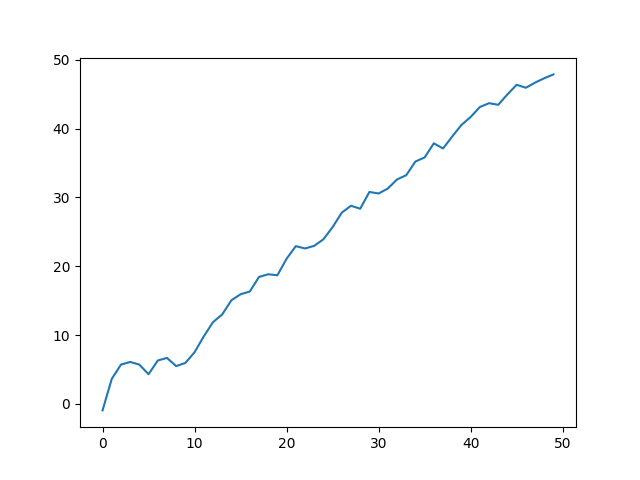
\includegraphics[width=20em]{tser_kf_02.png}

Kaynaklar

[1] Gelb, {\em Applied Optimal Estimation}

[2] Brown, osf. 143, {\em Introduction to Random Signals and Applied Kalman Filtering}

[3] Hartley, Zisserman, {\em Multiple View Geometry} 

[4] Labbe, {\em Kalman and Bayesian Filters in Python}

[5] Bayramli, Zaman Serileri, {\em Ortalamaya Dönüş ile İşlem}

\end{document}

